%! TeX root = report.tex

\section{\SpecFour{}: Two chains in \tlap{}}\label{sec:spec4}

We obtain this specification by preserving the vote and checkpoint behavior from \SpecThree{}, but we restrict the block-graph to exactly two chains, which are allowed to fork, i.e., they always share a common prefix.
To this end, we restrict block bodies of the two chains as follows:
\begin{enumerate}
	\item Block bodies on the first chain have non-negative sequential integer numbers starting from 0 (genesis), e.g. $0, 1, 2,3, 4$.
	\item Block bodies on the second chain are the same as the ones on the first chain \emph{up to the fork point}, after which they change sign, but otherwise maintain their sequence in absolute value terms, e.g. $0, 1,2,-3,-4$.
\end{enumerate}

The aim of this encoding is to decrease complexity for the SMT solver, since it simplifies block graph ancestry and closure reasoning significantly (e.g. we can check whether one block is an ancestor of another by simply comparing block body integer values), while preserving the behavior which arises from voting on checkpoint justification.

\subsection{Inductive Invariant}\label{sec:spec4-indinv}

This specification defines an inductive invariant \textit{IndInv}. Recall, an inductive invariant satisfies the following two conditions, assuming we have an initial-state predicate \textit{Init}, and transition predicate \textit{Next}:
\begin{enumerate}
	\item It is implied by the initial state: $\mathit{Init} \Rightarrow \mathit{IndInv}$
	\item It is preserved by the transition predicate: $\mathit{IndInv} \land \mathit{Next} \Rightarrow \mathit{IndInv}$
\end{enumerate}
Because of this characterization, inductive invariants lend themselves especially nicely to bounded symbolic model checking; with Apalache, one can prove (or disprove) an inductive invariant by running two queries of depth at most 1, corresponding to the above properties.
If no violation is found, we are assured that \textit{IndInv} holds in all possible reachable states.
Since our goal is ultimately to prove or disprove \textit{AccountableSafety}, we can additionally prove $\mathit{IndInv} \Rightarrow \mathit{AccountableSafety}$.

The challenge, typically, is that inductive invariants are more difficult to write, compared to state invariants.
They are usually composed of several lemmas, i.e. properties that we are less interested in on their own, but which are crucial in establishing property (2.).

As we explain below, the inductive invariant introduced in \SpecFour{} mainly consists of two sets of lemmas, one for characterizing the chain-fork scenarios, and a second one for characterizing justified checkpoints, shown in Figure~\ref{figFork} and Figure~\ref{figJC} respectively.

\begin{figure}
  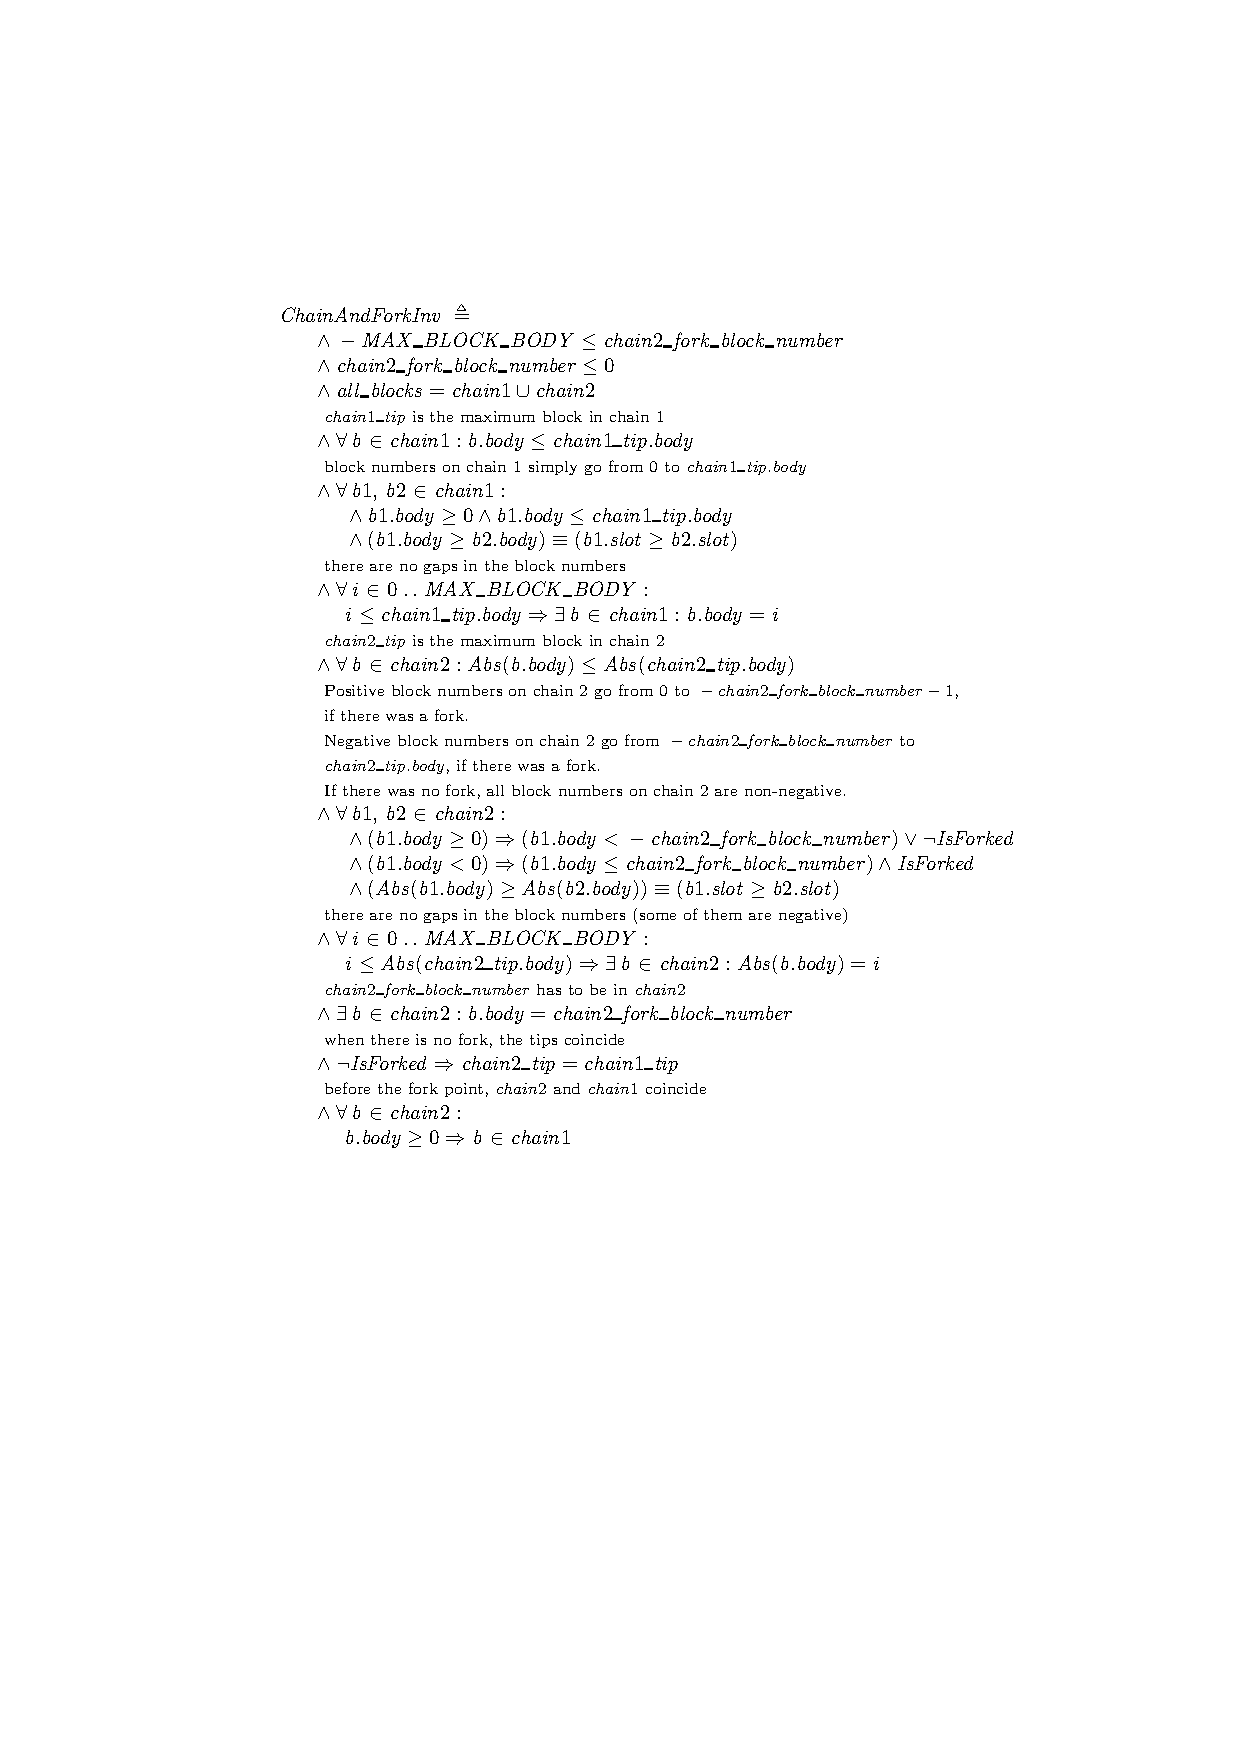
\includegraphics[width=\textwidth]{images/chain-and-fork-inv.pdf}
  \caption{Chain and forking lemmas in \textit{IndInv}}\label{figFork}
\end{figure}

\begin{figure}
  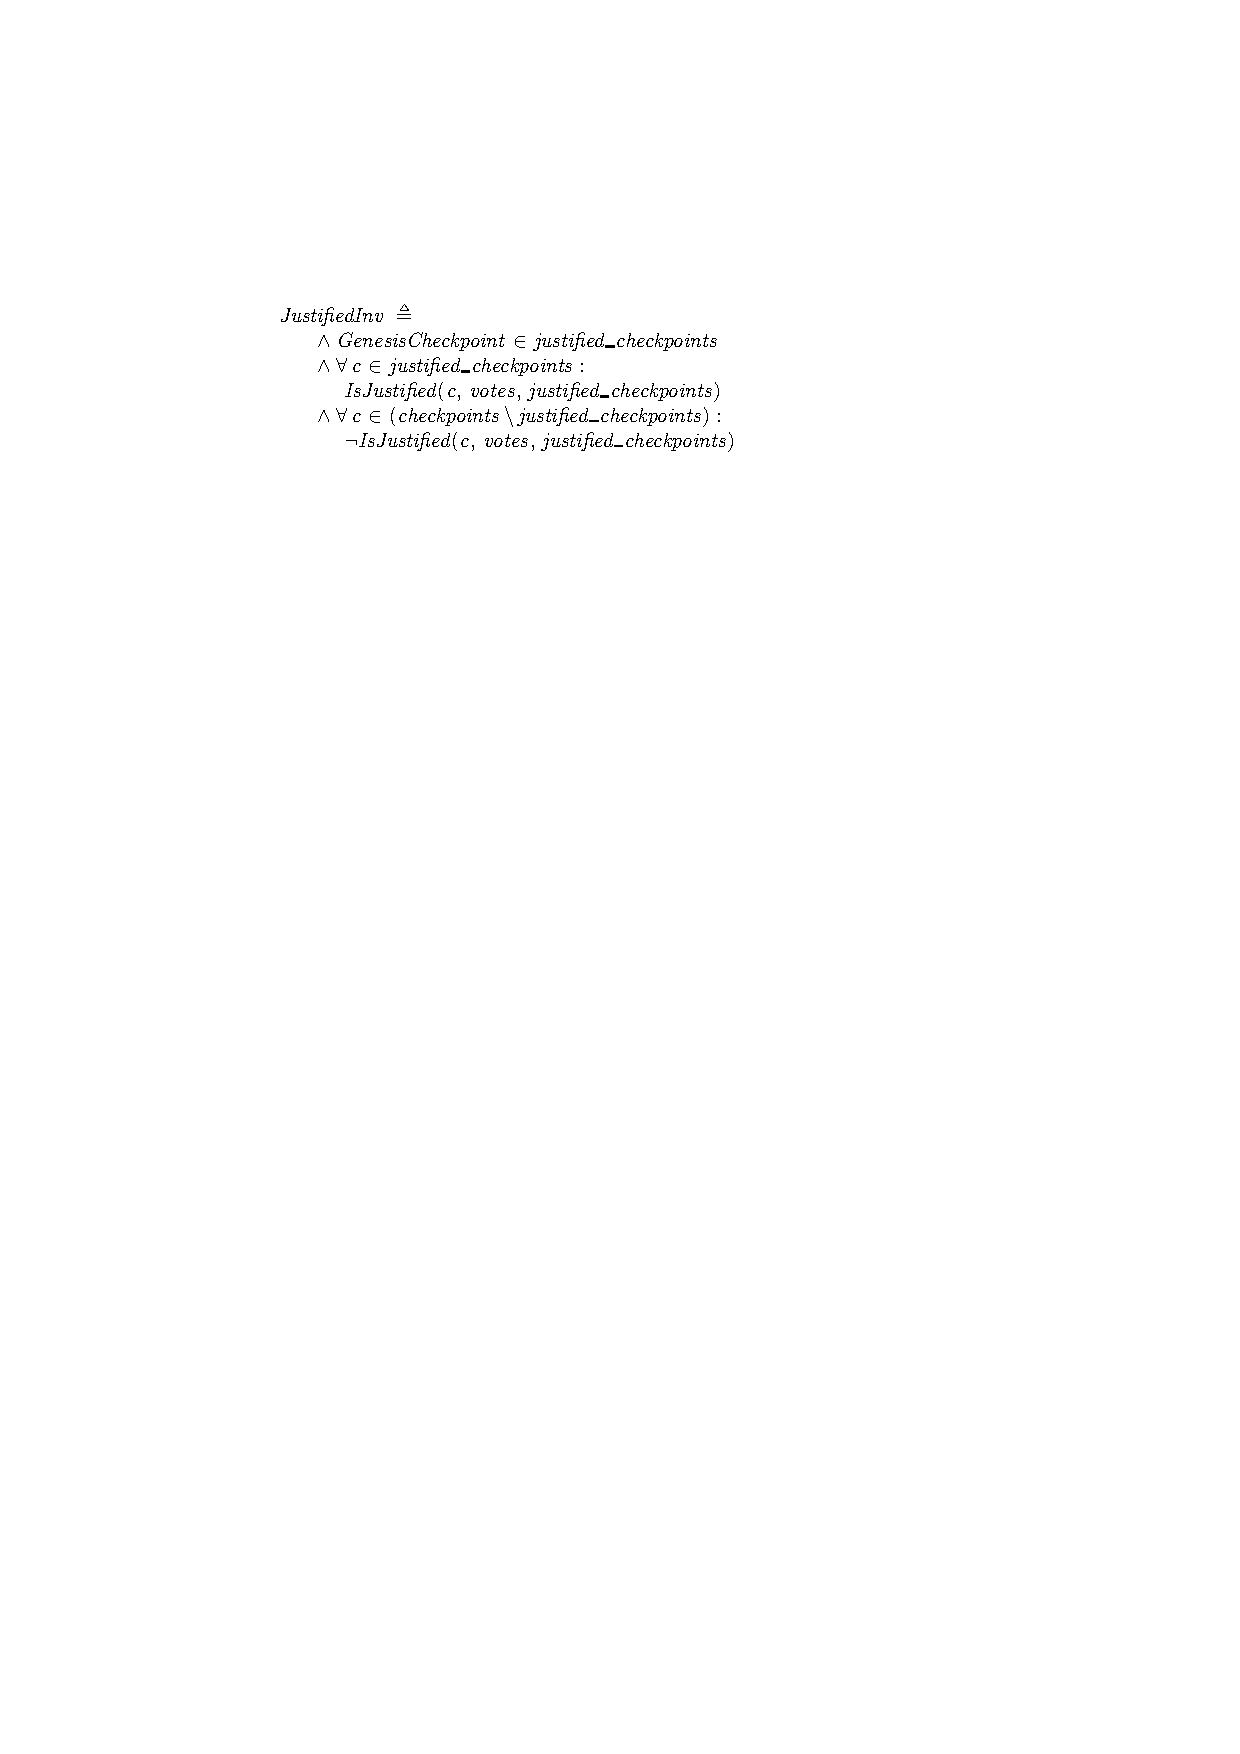
\includegraphics[width=\textwidth]{images/justified-inv.pdf}
  \caption{Justified checkpoint lemmas in \textit{IndInv}}\label{figJC}
\end{figure}

Since we represent a fork by means of a sign-change on block numbers, we have to specify that their absolute values are contiguous, that the chains coincide in the absence of a fork, as well as on the pre-fork prefix, and that both chains are monotone w.r.t. block numbers after the fork point.
Additionally, we require validity predicates for the vote set and checkpoints, as well as a precise characterization of the set of justified checkpoints. The latter merits further discussion.

\paragraph{Justified checkpoints.} To accurately describe the set of all justified checkpoints, we require two constraints:
\begin{enumerate}
	\item Consistency: Every checkpoint in the set is justified, and 
	\item Completeness: Every justified checkpoint belongs to the set.
\end{enumerate}
It is worth noting that both of these properties are required for an inductive invariant; if we do not specify consistency, the solver can trivially infer that the set contains all possible checkpoints, and that all checkpoints are finalized, which leads to bogus counterexamples to \textit{AccountableSafety}.
On the other hand, if we don't specify completeness, the solver can trivially infer that the set of justified checkpoints is empty (or contains exactly the genesis checkpoint). This leads us to be unable to detect real violations of \textit{AccountableSafety}, since we can never observe conflicting finalized checkpoints, even when the votes cast necessitate their existence.

This is critical, because including both constraints places a heavy burden on the solver. No matter how we define the justification predicate, it will inevitably appear in both positive and negative form, forcing the solver to contend with both quantifier alternations and double universal quantification, both of which are known to be hard.
Fundamentally, this demonstrates the intrinsic complexity of the problem itself, regardless of the particular characterization of justified sets in \tlap{}.

\subsection{Model checking experiments}

Table~\ref{tab:spec4-experiments} summarizes our experiments on checking
inductiveness and accountable safety of~\SpecFourB{}. Interestingly, checking
inductiveness of~\texttt{IndInv} takes seconds. However,
checking~\texttt{AccountableSafety} against the inductive invariant times out.

\begin{table}
    \centering
    \begin{tabular}{lllrrr}
            \tbh{Init}
            & \tbh{Step}
            & \tbh{Invariant}
            & \tbh{Depth}
            & \tbh{Memory}
            & \tbh{Time}
            \\ \toprule
            \texttt{Init}
            & \texttt{Next}
            & \texttt{IndInv}
            & 0
            & 0.6 GB
            & 2sec
            \\
            \texttt{IndInit}
            & \texttt{Next}
            & \texttt{IndInv}
            & 1
            & 0.6 GB
            & 2sec
            \\
            \texttt{IndInit}
            & \texttt{Next}
            & \texttt{AccountableSafety}
            & 0
            & 1.5 GB
            & TO ($> 6$d)
            \\
            \bottomrule
    \end{tabular}
    \caption{Model checking experiments
        with~\SpecFour{} on the instance~\texttt{MC\_ffg\_b3\_ffg5\_v12}
        (``TO'' means timeout)
    }\label{tab:spec4-experiments}
\end{table}

